\section{Biological background}
\label{sec:biol-backgr}

-disease states and bio cond are character by distinct gene expression (DeRisis 1997; spellman 1998; Eisen and Brown
1999; Brown Botstein 1999)

\subsection{RNA sequencing}
\label{sec:rna-sequencing}

Ever since the mid to late nineties the importance of expression of individual genes in determining biological condition
and {\color{red} likelihood of} disease. Until recently the most prevalent method for obtaining 

\begin{figure}
  \centering
  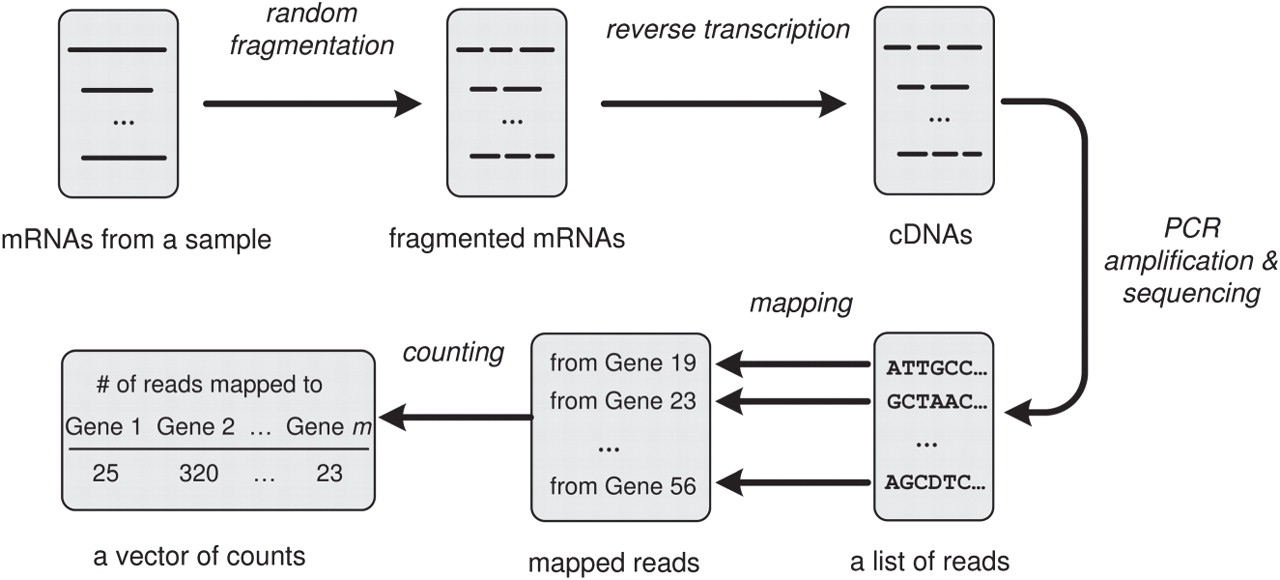
\includegraphics[width=0.9\textwidth]{pics/li-biostats12.jpg}
  \caption{Figure from Li et al., Normalization, testing, and false discovery rate estimation for RNA-sequencing data, Biostatistics, 2012, 13(3), by permission of Oxford University Press.}
  \label{fig:li-biostats}
\end{figure}


%%% Local Variables:
%%% TeX-master: "warwickthesis"
%%% End:
